% !TEX program = xelatex
% Шаблон научной статьи НИТУ «МИСиС»
% Заполните блоки ниже и скомпилируйте: xelatex article.tex

\documentclass{misisarticle}

% --- Классификационные коды (оставьте пустым {}, если не требуются) ---
\grnti{28.23.15; 28.23.23; 73.31.11}
\asjc{1707, 1702, 2215, 3313}
\oecd{1.02}

% --- Название ---
\title{Сравнительное исследование эффективности нейросетевых моделей при прогнозировании движения пешеходов перед общественным рельсовым транспортом}

% --- Авторы: \misisauthor{ФИО}{аффилиация}{город, страна}{email} ---
\misisauthor{М.~И.~Фейгенберг}{кафедра инженерной кибернетики НИТУ «МИСиС»}{Москва, Россия}{m2311505@edu.misis.ru}
\misisauthor{Р.~Н.~Садеков}{кафедра инженерной кибернетики НИТУ «МИСиС»}{Москва, Россия}{sadekov@misis.ru}

% --- Аннотация и ключевые слова ---
\abstract{%
  Рассматривается задача прогнозирования траекторий движения пешеходов по ходу следования городского рельсового транспорта. В условиях большой массы состава, невозможности бокового маневрирования и ограничений на рывок при торможении (для безопасности стоящих пассажиров) критически важно заблаговременное обнаружение риска наезда. Существующие кинематические и базовые рекуррентные модели накапливают ошибку на горизонтах свыше 1 секунды и приводят к частым ложным тревогам, игнорируя намерения человека и динамику самого транспорта. Проводится сравнительное исследование эффективности линейных экстраполяторов, классических сетей LSTM и мультимодальной нейросетевой модели с двухуровневым механизмом внимания (пространственным и временным), комплексирующей историю координат пешехода, визуальный контекст его намерения перейти пути и вектор скорости подвижного состава. Проверка моделей проводится на открытом бенчмарке и натурных видеозаписях с фронтальной камеры трамвая. Оценка качества выполняется по метрикам средней ошибки смещения (CMSE), ошибки конечной точки (CFMSE), времени инференса и расчетному запасу времени до столкновения (TTC).
}

\keywords{%
  прогнозирование траектории; городской рельсовый транспорт; коридор динамического габарита; оценка риска столкновения; рекуррентные нейронные сети
}

\begin{document}

\maketitle

% ============================================================
\section{Введение}

Городской рельсовый транспорт функционирует в условиях плотного смешанного транспортного потока крупных мегаполисов. В отличие от изолированных линий метрополитена и железных дорог, трамвайные пути в центральных районах городов проложены непосредственно по проезжей части или на совмещенном полотне вдоль бульваров и пешеходных зон. В таких условиях пешеходы, пассажиры и автомобильный транспорт постоянно взаимодействуют в едином пространстве. Остановочные пункты нередко располагаются посередине улицы, поэтому посадка и высадка пассажиров сопряжены с нерегулируемым пересечением проезжей части и рельсового полотна~\cite{kustenko2025}.

Актуальность задачи заблаговременного предотвращения столкновений в рельсовом транспорте обусловлена физико-механическими особенностями движения вагона. Масса современного низкопольного трехсекционного трамвайного вагона составляет от 28 до 42 тонн, а жесткость стального кузова многократно превосходит конструкцию легкового автомобиля. Коэффициент сцепления стального колеса со стальным рельсом при сухой погоде составляет $\mu \approx 0{,}15\dots0{,}18$, а при дожде, обледенении или попадании влажной листвы падает до $\mu \approx 0{,}07\dots0{,}09$~\cite{lewis2009}. Вследствие этого тормозной путь вагона при скорости $40$~км/ч на влажном пути превышает $35$--$40$~метров. Принципиальным динамическим ограничением трамвая является невозможность совершения бокового маневра для объезда препятствия: рельсовый транспорт жестко зафиксирован в колее, а предельное замедление при служебном торможении ограничено допустимым рывком во избежание падения стоящих пассажиров в салоне.

Существующие автомобильные системы содействия водителю (ADAS)~\cite{gost70249} и комплексы автономного вождения не могут быть напрямую перенесены на городской рельсовый транспорт. Автомобильные алгоритмы проектируются в расчете на высоту установки камеры $1{,}2$--$1{,}4$~м от дорожного полотна, предполагают возможность перестроения транспортного средства и опираются на открытые наборы данных, лишенные специфики рельсовой колеи и габаритов приближения строений~\cite{gost9238}. Гарантированное предотвращение наезда требует заблаговременного прогнозирования траектории движения пешехода на горизонте от $2{,}5$ до $3{,}5$~секунд.

Целью настоящей работы является исследование и сопоставление алгоритмических подходов к краткосрочному и среднесрочному прогнозированию движения пешеходов перед движущимся трамваем по данным монокулярного видеопотока и бортовой телеметрии. Планируется сравнительная оценка кинематических и нейросетевых методов прогнозирования траекторий пешеходов по точности предсказания координат и своевременности оценки риска наезда в створе рельсового пути. Предполагаемый вклад работы заключается в выявлении влияния динамики подвижного состава и оптического параллакса на погрешность прогнозирования на различных горизонтах упреждения, а также в формулировании рекомендаций по выбору моделей и пороговых параметров для бортовых систем активной безопасности трамвая.

% ============================================================
\section{Анализ существующих исследований}

Задача прогнозирования движения участников дорожной сцены и оценки пространственной обстановки активно исследуется в современной научной литературе~\cite{rudenko2020}. В сфере рельсового транспорта методы глубокого обучения и трехмерного детектирования объектов успешно применяются для предсказания поведения транспортных средств в дорожной сцене перед автономным трамваем~\cite{guzhva2022}. В смежных работах исследуются алгоритмы построения карты пространства с высоты птичьего полета (BEV) по видеопоследовательности с монокулярной камеры, включая тестирование на натурных видеозаписях из кабины трамвая~\cite{kozhukhov2023}, а также методы оценки проходимости пути и выделения препятствий по монокулярному видеопотоку~\cite{vasilchikov2026}.

Методы непосредственного прогнозирования траекторий пешеходов можно разделить на четыре основные группы.

\subsection{Физико-кинематические экстраполяторы}

Детерминированные кинематические модели опираются на гипотезу о сохранении постоянной скорости (Constant Velocity, CV) или постоянного ускорения (Constant Acceleration, CA). Для фильтрации шума детектора и оценки вектора скорости применяется дискретный линейный фильтр Калмана~\cite{kalman1960}. Главным достоинством подхода является минимальная вычислительная задержка (менее $3$~мс на CPU). Однако линейные экстраполяторы не учитывают социальные взаимодействия и намерения человека: при резком начале перехода или остановке перед путями модель накапливает значительную ошибку на горизонтах свыше $1$~секунды.

\subsection{Классические рекуррентные нейронные сети}

Для учета истории перемещений и нелинейной динамики в компьютерном зрении получили распространение сети долгой краткосрочной памяти (LSTM). В модели Social-LSTM~\cite{alahi2016} каждому пешеходу сопоставляется индивидуальный рекуррентный модуль, а взаимодействие между людьми моделируется через слой социального пулинга скрытых состояний. Несмотря на способность аппроксимировать сложные траектории, базовые LSTM-сети страдают от накопления ошибки при авторегрессионном декодировании и не учитывают визуальные признаки намерения пешехода и собственное движение камеры.

\subsection{Пространственно-временные графовые и вероятностные сети}

Развитием методов моделирования толпы стали пространственно-временные графовые сверточные сети, такие как Social-STGCNN~\cite{mohamed2020}, где сцена представляется в виде графа, а временная динамика обрабатывается сверточными слоями TCN. В классе мультимодальных вероятностных генераторов эталонным решением выступает архитектура Trajectron++~\cite{salzmann2020}, использующая условный вариационный автоэнкодер (CVAE) с внедрением дифференцируемого кинематического слоя и растровых семантических карт. Для моделирования совместного внимания по времени и агентам также применяются трансформерные модели, такие как AgentFormer~\cite{yuan2021}.

\subsection{Мультимодальные модели с оценкой намерения и механизмами внимания}

Принципиальным ограничением алгоритмов, использующих только координаты ограничивающих рамок (BBox), является запаздывание реакции на старт движения человека. Перед выходом на пути пешеход поворачивает голову, меняет наклон корпуса и шаг. В работе Rasouli и соавт.~\cite{rasouli2019} предложен датасет и мультимодальная архитектура PIEPredict с механизмами временного и пространственного внимания, которая комплексирует историю координат BBox, визуальный контекст намерения перейти проезжую часть (Crossing Intent) и вектор скорости самого транспортного средства. Учет визуального намерения и скорости подвижного состава позволяет снизить число ложных срабатываний на остановочных платформах, где пассажиры находятся в непосредственной близости от габарита вагона без намерения пересекать пути.

% ============================================================
\section{Постановка задачи}

\subsection{Динамика торможения и коридор динамического габарита}

Процесс торможения трамвайного вагона включает три фазы: время восприятия и вычислительной задержки распознавания $\tau_{\text{реакц}}$ ($0{,}3$--$0{,}8$~с), время срабатывания тормозного привода $\tau_{\text{прив}}$ ($0{,}2$--$0{,}4$~с) и установившееся замедление $a_{\text{торм}} = g \cdot \mu_{\text{сцеп}}$. Полный остановочный путь вагона $S_{\text{остан}}$ при начальной скорости $v_0$ определяется выражением:
\begin{equation}
  S_{\text{остан}}(v_0) = v_0 \cdot (\tau_{\text{реакц}} + \tau_{\text{прив}}) + \frac{v_0^2}{2 \cdot a_{\text{торм}}}.
  \label{eq:stop_dist}
\end{equation}

На рис.~\ref{fig:stopping} приведены расчетные кривые полного остановочного пути трамвая в зависимости от скорости и состояния рельсов. При скорости $40$~км/ч ($11{,}11$~м/с) остановочный путь возрастает с $43{,}8$~м на сухом рельсе до $88{,}0$~м на влажном рельсе, что диктует необходимость прогнозирования траекторий на горизонте $T_{\text{pred}} = 2{,}5\dots3{,}5$~с.

\begin{figure}[htbp]
  \centering
  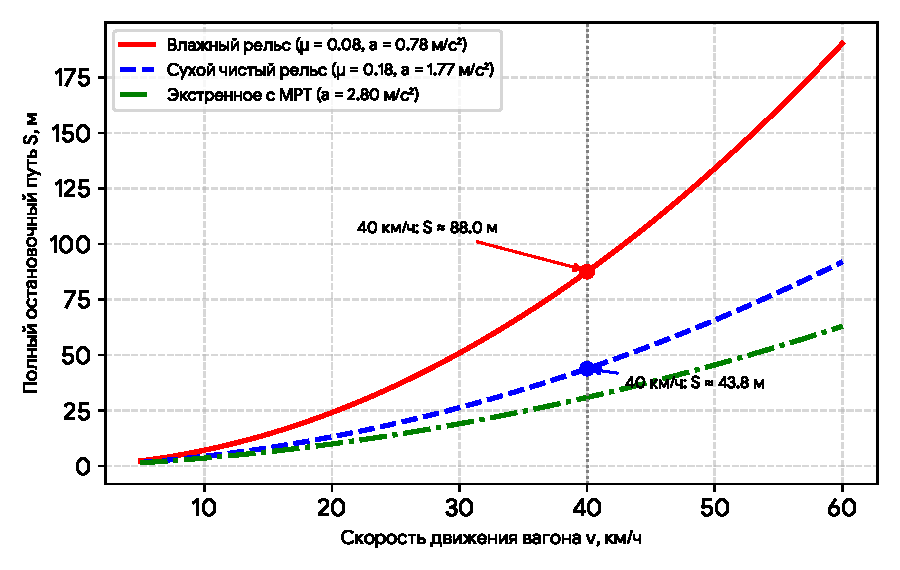
\includegraphics[width=0.98\columnwidth]{figures/stopping_distance.pdf}
  \caption{Зависимость полного остановочного пути трамвая от скорости движения при различных состояниях рельсового полотна.}
  \label{fig:stopping}
\end{figure}

Согласно ГОСТ 9238--2013~\cite{gost9238}, номинальная ширина кузова вагона $B_{\text{вагона}}$ составляет $2{,}50$--$2{,}65$~м. С учетом бокового защитного интервала $\delta_{\text{safe}} = 0{,}25$--$0{,}35$~м ширина коридора динамического габарита вдоль оси рельсового пути составляет:
\begin{equation}
  W_{\text{clear}} = B_{\text{вагона}} + 2 \cdot \delta_{\text{safe}} \approx 3{,}0\dots3{,}2~\text{м}.
  \label{eq:wclear}
\end{equation}

Пусть $(x_{\text{ped}}(t), y_{\text{ped}}(t))$~--- поперечная и продольная координаты пешехода в системе координат пути (ось пути соответствует $x_{\text{rail}} = 0$), а $y_{\text{tram}}(t)$~--- продольная координата переднего бампера трамвая. Факт возникновения риска наезда $C(t, T_{\text{pred}}) \in \{0, 1\}$ на горизонте $\tau \in [t, t + T_{\text{pred}}]$ формализуется как одновременное вхождение пешехода в коридор динамического габарита на дистанции менее остановочного пути:
\begin{equation}
  C(t, T_{\text{pred}}) = 1 \Leftrightarrow \exists \tau \in [t, t + T_{\text{pred}}]:
  \begin{cases}
    |x_{\text{ped}}(\tau) - x_{\text{rail}}| \le \dfrac{W_{\text{clear}}}{2}, \\
    d_{\text{long}}(\tau) \le S_{\text{остан}}(v_{\text{tram}}(\tau)),
  \end{cases}
  \label{eq:collision}
\end{equation}
где $d_{\text{long}}(\tau) = y_{\text{ped}}(\tau) - y_{\text{tram}}(\tau)$~--- продольная дистанция до пешехода. Расчетный запас времени до столкновения (Time-to-Collision, TTC) вычисляется по формуле:
\begin{equation}
  TTC(t) = \frac{d_{\text{long}}(t)}{v_{\text{tram}}(t) + v_{\text{ped}}^{\text{long}}(t)},
  \label{eq:ttc}
\end{equation}
где $v_{\text{ped}}^{\text{long}}(t)$~--- проекция скорости пешехода на продольную ось пути (положительна при встречном движении).

\subsection{Оптико-геометрическая модель и оптический параллакс}

Бортовая камера монтируется в кабине трамвая на высоте $H_{\text{cam}} \approx 2{,}8\dots3{,}2$~м с наклоном оптической оси вниз ($\theta \approx -8^\circ\dots-14^\circ$). Поскольку стопы пешехода контактируют с плоскостью рельсового полотна ($Z_w = 0$), переход от пиксельных координат середины нижнего края рамки пешехода $(u_{\text{ног}}, v_{\text{ног}})$ к мировым координатам на плоскости пути $(X_w, Y_w)$ задается невырожденным преобразованием плоской гомографии $H \in \mathbb{R}^{3 \times 3}$~\cite{hartley2004}:
\begin{equation}
  \begin{pmatrix} X_w \\ Y_w \\ 1 \end{pmatrix} \sim H^{-1} \begin{pmatrix} u_{\text{ног}} \\ v_{\text{ног}} \\ 1 \end{pmatrix}, \quad H = K \begin{pmatrix} r_1 & r_2 & t \end{pmatrix},
  \label{eq:homography}
\end{equation}
где $K$~--- матрица внутренних параметров камеры, $r_1, r_2$~--- столбцы матрицы вращения, $t$~--- вектор переноса.

Наблюдаемое в кадре смещение пешехода складывается из его физического движения со скоростью $v_{\text{ped}}$ и оптического параллакса, вызванного собственным движением трамвая со скоростью $v_{\text{tram}}(t)$ и угловой скоростью $\omega(t)$:
\begin{equation}
  X_c(t + \Delta t) = R_{\text{tram}}(\Delta t) X_c(t) + T_{\text{tram}}(v_{\text{tram}}, \Delta t) + v_{\text{ped}} \Delta t.
  \label{eq:parallax}
\end{equation}

Без подачи вектора скорости подвижного состава $v_{\text{tram}}(t)$ в модель прогнозирования замедление или ускорение вагона искажает наблюдаемый оптический поток и вызывает систематический снос предсказанной траектории.

% ============================================================
\section{Методы и организация исследования}

\subsection{Сравниваемые модели прогнозирования}

В рамках планируемого вычислительного эксперимента сопоставляются четыре модельные конфигурации, отражающие эволюцию от кинематических фильтров к мультимодальным сетям с вниманием (табл.~\ref{tab:models}):
\begin{itemize}
  \item \textbf{Линейный экстраполятор (CV + фильтр Калмана):} базовая кинематическая модель, оценивающая вектор состояния $[x, y, \dot{x}, \dot{y}]^T$ по истории координат точки опоры ног пешехода.
  \item \textbf{Классическая сеть LSTM:} рекуррентная архитектура типа Encoder-Decoder, принимающая последовательность наблюдаемых координат пешехода за интервал истории $T_{\text{obs}} = 0{,}8$--$1{,}5$~с и регрессирующая будущие смещения без учета визуального контекста.
  \item \textbf{Пространственно-временная графовая сеть (Social-STGCNN):} графовая сверточная модель~\cite{mohamed2020}, оценивающая параметры двумерного распределения Гаусса координат пешеходов с учетом взаимного расположения людей на посадочной платформе.
  \item \textbf{Мультимодальная модель с двухуровневым вниманием (PIEPredict-Rail):} адаптированная архитектура~\cite{rasouli2019} с пространственным и временным механизмами внимания, комплексирующая историю координат BBox, визуальные признаки намерения человека перейти пути (по локальному кропу изображения) и вектор скорости подвижного состава $v_{\text{tram}}(t)$ с добавлением геометрического штрафа за ложное пересечение границ коридора габарита $W_{\text{clear}}$.
\end{itemize}

\begin{table}[htbp]
  \caption{Конфигурации исследуемых моделей прогнозирования}
  \label{tab:models}
  \centering
  \begin{tabular}{p{0.26\columnwidth}p{0.34\columnwidth}p{0.28\columnwidth}}
    \toprule
    \textbf{Модель} & \textbf{Входные модальности} & \textbf{Учет динамики и колеи} \\
    \toprule
    CV + Калман & 2D/3D координаты стоп & Нет (линейная инерция) \\
    Классическая LSTM & История координат BBox & Нет (только кинематика трека) \\
    Social-STGCNN & Пространственный граф треков & Косвенный (через граф связей) \\
    Мультимодальная (Attention) & BBox, визуальный контекст намерения, вектор $v_{\text{tram}}$ & Прямой (эго-скорость + коридор габарита) \\
    \bottomrule
  \end{tabular}
\end{table}

\subsection{Используемые данные и протокол оценки качества}

Для обеспечения воспроизводимости и всесторонней проверки исследование опирается на два источника данных:
\begin{itemize}
  \item \textbf{Открытый бенчмарк PIE (Pedestrian Intention Estimation):} содержит размеченные городские видеопоследовательности с аннотациями ограничивающих рамок, меток намерения перехода и телеметрии скорости транспортного средства~\cite{rasouli2019}.
  \item \textbf{Натурные видеозаписи с фронтальной камеры трамвая:} тестовый набор видеозаписей высокого разрешения (Full HD, $30$~FPS), снятых из кабины трамвая на действующем московском маршруте (включая зоны остановочных пунктов, совмещенного полотна и нерегулируемых переходов). Видеоданные сопровождаются разметкой ограничивающих прямоугольников BBox (выполненной с использованием детектора YOLO и трекера ByteTrack~\cite{zhang2022} с ручной верификацией), координатами точек контакта стоп для проекции через плоскую гомографию~\eqref{eq:homography} и профилем скорости движения состава.
\end{itemize}

Оценка качества моделей на горизонтах прогнозирования от $0{,}5$ до $3{,}0$~с выполняется по четырем целевым показателям:
\begin{enumerate}
  \item \textbf{Средняя ошибка смещения (CMSE / ADE)}~--- среднеквадратичное (или среднее евклидово) отклонение предсказанных координат центроида/точки опоры пешехода $\hat{p}_t^i$ от истинных координат $p_t^i$ по всем $N$ пешеходам и шагам горизонта прогнозирования от $T_{\text{obs}}+1$ до $T_{\text{pred}}$:
  \begin{equation}
    CMSE = \frac{1}{N (T_{\text{pred}} - T_{\text{obs}})} \sum_{i=1}^{N} \sum_{t=T_{\text{obs}}+1}^{T_{\text{pred}}} \|\hat{p}_t^i - p_t^i\|_2^2.
    \label{eq:cmse}
  \end{equation}
  \item \textbf{Ошибка конечной точки (CFMSE / FDE)}~--- квадратичная ошибка смещения в финальной точке горизонта упреждения $t = T_{\text{pred}}$:
  \begin{equation}
    CFMSE = \frac{1}{N} \sum_{i=1}^{N} \|\hat{p}_{T_{\text{pred}}}^i - p_{T_{\text{pred}}}^i\|_2^2.
    \label{eq:cfmse}
  \end{equation}
  \item \textbf{Время инференса}~--- средняя вычислительная задержка прямого прохода модели на один кадр (мс), определяющая пригодность алгоритма для работы в реальном времени на бортовом вычислителе.
  \item \textbf{Расчетный запас времени до столкновения (TTC)}~--- точность и своевременность обнаружения критического сближения по формулам~\eqref{eq:collision}--\eqref{eq:ttc}, оцениваемая через долю верных предупреждений и частоту ложных тревог на остановочных платформах.
\end{enumerate}

На текущем этапе исследования сформированы теоретико-множественная и оптико-геометрическая модели системы, подготовлена спецификация разметки трамвайных видеозаписей и определен протокол сравнительных испытаний; экспериментальная верификация численных значений метрик на полном корпусе маршрутных записей запланирована в качестве следующего шага работы.

% ============================================================
\begin{thebibliography}{99}

\bibitem{kustenko2025} Кустенко А.~А., Капский Д.~В., Ларин О.~Н. Моделирование движения транспортных средств в местах посадки пассажиров в трамвай с проезжей части // Транспорт Урала. --- 2025. --- №~2~(85). --- С.~22--28.

\bibitem{lewis2009} Lewis R., Olofsson U. \textit{Wheel-Rail Interface Handbook}. --- Cambridge: Woodhead Publishing, 2009. --- 792~p.

\bibitem{gost70249} ГОСТ Р 70249--2022. Системы искусственного интеллекта на автомобильном транспорте. Высокоавтоматизированные транспортные средства. Термины и определения. --- М.: ФГБУ «РСТ», 2022. --- 24~с.

\bibitem{gost9238} ГОСТ 9238--2013. Габариты железнодорожного подвижного состава и приближения строений. --- М.: Стандартинформ, 2014. --- 172~с.

\bibitem{rudenko2020} Rudenko A., Palmieri L., Herman M., Kitani K.~M., Gavrila D.~M., Arras K.~O. Human motion trajectory prediction: a survey // The International Journal of Robotics Research. --- 2020. --- Vol.~39, no.~8. --- P.~895--935.

\bibitem{guzhva2022} Guzhva N.~S., Prun V.~E., Postnikov V.~V., Lobanov M.~G., Sadekov R.~N., Sholomov D.~L. Using 3D Object Detection DNN in an Autonomous Tram to Predict the Behaviour of Vehicles in the Road Scene // 2022 29th Saint Petersburg International Conference on Integrated Navigation Systems (ICINS). --- Saint Petersburg, 2022. --- P.~1--6.

\bibitem{kozhukhov2023} Кожухов А.~А., Хонер П.~Д. Построение карты пространства вокруг автомобиля на основе видеопоследовательности // Искусственный интеллект в промышленных, коммерческих, медицинских и финансовых приложениях: сборник статей научно-технического семинара студентов кафедры «Инженерной кибернетики». Вып.~1 / Под ред. А.~Р.~Ефимова. --- М.: НИТУ «МИСИС», 2023. --- С.~22--27.

\bibitem{vasilchikov2026} Васильчиков А.~В. Оценка проходимости пути по монокулярному видеопотоку с использованием нейросетевой сегментации и относительной глубины сцены // Искусственный интеллект в промышленных, коммерческих, медицинских и финансовых приложениях: сборник статей научно-технического семинара. Вып.~6 / Под ред. А.~Р.~Ефимова. --- М.: НИТУ «МИСИС», 2026. --- С.~11--15.

\bibitem{kalman1960} Kalman R.~E. A New Approach to Linear Filtering and Prediction Problems // Journal of Basic Engineering. --- 1960. --- Vol.~82, no.~1. --- P.~35--45.

\bibitem{alahi2016} Alahi A., Goel K., Ramanathan V., Robicquet A., Fei-Fei L., Savarese S. Social LSTM: Human Trajectory Prediction in Crowded Spaces // Proceedings of the IEEE Conference on Computer Vision and Pattern Recognition (CVPR). --- 2016. --- P.~961--971.

\bibitem{mohamed2020} Mohamed A., Qian K., Elhoseiny M., Claudel C. Social-STGCNN: A Social Spatio-Temporal Graph Convolutional Neural Network for Human Trajectory Prediction // Proceedings of the IEEE/CVF Conference on Computer Vision and Pattern Recognition (CVPR). --- 2020. --- P.~14412--14420.

\bibitem{salzmann2020} Salzmann T., Ivanovic B., Chakravarty P., Pavone M. Trajectron++: Dynamically-Feasible Trajectory Forecasting with Heterogeneous Data // Computer Vision -- ECCV 2020. Lecture Notes in Computer Science. --- Springer, Cham, 2020. --- Vol.~12363. --- P.~683--700.

\bibitem{yuan2021} Yuan Y., Weng X., Ou Y., Kitani K. AgentFormer: Agent-Aware Transformers for Socio-Temporal Multi-Agent Forecasting // Proceedings of the IEEE/CVF International Conference on Computer Vision (ICCV). --- 2021. --- P.~9793--9803.

\bibitem{rasouli2019} Rasouli A., Kotseruba I., Kunic T., Tsotsos J.~K. PIE: A Large-Scale Dataset and Models for Pedestrian Intention Estimation and Trajectory Prediction // Proceedings of the IEEE/CVF International Conference on Computer Vision (ICCV). --- 2019. --- P.~6261--6270.

\bibitem{hartley2004} Hartley R., Zisserman A. \textit{Multiple View Geometry in Computer Vision}. --- 2nd ed. --- Cambridge: Cambridge University Press, 2004. --- 655~p.

\bibitem{zhang2022} Zhang Y., Sun P., Jiang Y., Yu D., Weng F., Yuan Z., Luo P., Liu W., Wang X. ByteTrack: Multi-Object Tracking by Associating Every Detection Box // Computer Vision -- ECCV 2022. Lecture Notes in Computer Science. --- Springer, Cham, 2022. --- Vol.~13682. --- P.~1--21.

\end{thebibliography}

\end{document}
